\let\negmedspace\undefined
\let\negthickspace\undefined
\documentclass[journal]{IEEEtran}
\usepackage[a5paper, margin=10mm, onecolumn]{geometry}
%\usepackage{lmodern} % Ensure lmodern is loaded for pdflatex
\usepackage{tfrupee} % Include tfrupee package

\setlength{\headheight}{1cm} % Set the height of the header box
\setlength{\headsep}{0mm}     % Set the distance between the header box and the top of the text

\usepackage{gvv-book}
\usepackage{gvv}
\usepackage{cite}
\usepackage{amsmath,amssymb,amsfonts,amsthm}
\usepackage{algorithmic}
\usepackage{graphicx}
\usepackage{textcomp}
\usepackage{xcolor}
\usepackage{txfonts}
\usepackage{listings}
\usepackage{enumitem}
\usepackage{mathtools}
\usepackage{gensymb}
\usepackage{comment}
\usepackage[breaklinks=true]{hyperref}
\usepackage{tkz-euclide} 
\usepackage{listings}
% \usepackage{gvv}                                        
\def\inputGnumericTable{}                                 
\usepackage[latin1]{inputenc}                                
\usepackage{color}                                            
\usepackage{array}                                            
\usepackage{longtable}                                       
\usepackage{calc}                                             
\usepackage{multirow}                                         
\usepackage{hhline}                                           
\usepackage{ifthen}                                           
\usepackage{lscape}
\begin{document}

\bibliographystyle{IEEEtran}
\vspace{3cm}

\title{1.6.17}
\author{EE24BTECH11058 - P.Shiny Diavajna}
% \maketitle
% \newpage
% \bigskip
{\let\newpage\relax\maketitle}

\renewcommand{\thefigure}{\theenumi}
\renewcommand{\thetable}{\theenumi}
\setlength{\intextsep}{10pt} % Space between text and floats


\numberwithin{equation}{enumi}
\numberwithin{figure}{enumi}
\renewcommand{\thetable}{\theenumi}

\textbf{Question}:Using vectors,find the value of $k$ such that points $\myvec{k & -10 & 3}$, $\myvec{1 & -1 & 3}$ and $\myvec{3 & 5 & 3}$ are collinear.\\

\solution 
    
\begin{table}[h!]    
     \centering
     \begin{tabular}[12pt]{ |c| c|}
    \hline
    \textbf{Variable} & \textbf{Description}\\ 
    \hline
	$\myvec{k &-10 & 3}$ & Point $\vec{A}$\\
    \hline 
	$\myvec{1 & -1 & 3}$ & Point $\vec{B}$\\
    \hline
	$\myvec{3 & 5 & 3 }$ & Point $\vec{C}$\\
    \hline   
	$k$ & $x$ coordinate of $\vec{A}$\\
    \hline
    \end{tabular}

     \caption{Variables Used}
     \label{tab1.6.17.1}
   \end{table}

   \begin{align*}
     \myvec{C-B & B-A}^\top =\myvec{2 & 6 & 0 \\ 1-k & 9 & 0}\\
     \xrightarrow{R_2=R_1-\frac{6}{9}R_1} \myvec{2 & 6 & 0 \\ \frac{4+2k}{3} & 0 & 0}\\ 
   \end{align*} 

   \begin{align*}
     \frac{4+2k}{3} = 0 \\
        k=-2
    \end{align*}


   \begin{figure}[h!]
    \centering
    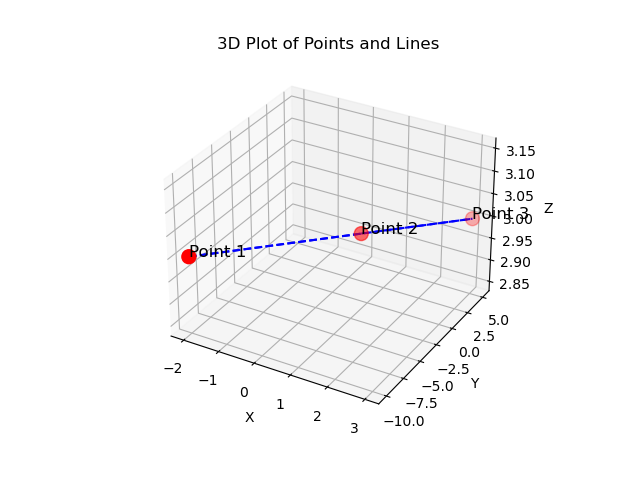
\includegraphics[width=0.7\linewidth]{figs/Figure_2.png}
    \caption{Plot for points A , B and C}
   \end{figure}
\end{document}
